\section{Scheduling para tiempo real}

Al analizar los algoritmos de scheduling, Tanembaum \cite[p.~136]{tanenbaum2001} señala que es relevante distinguir tres ambientes diferentes:

\begin{itemize}
	\item{Batch}
    
    \item{Interactivo}
    
    \item{Tiempo Real}
\end{itemize}

En los ambientes batch, no existe la exigencia planteada por los usuarios frente a alg\'un tipo de perif\'erico o terminal. Como no se necesita una respuesta interactiva r\'apida, son aceptables algoritmos sin desalojo o bien algoritmos con desalojo que tienen un quantum largo. Se requiere un uso intensivo y largo del CPU. Conviene entonces minimizar el overhead del cambio de contexto.

En el caso de los ambientes interactivos, lo que se intenta es que las tareas no acaparen el recurso CPU e impidan que otras tareas accedan a \'el. Por ello, conviene plantear una estrategia de desalojo.

El tercer ambiente es el que concierne al paper de Liu y Leilan \cite{liuleiland1973}: tiempo real. Se trata de ambientes en los que el control del tiempo de ejecuci\'on de cada proceso es cr\'itico. En estos ambientes \textbf{es necesario que la ejecuci\'on de cada tarea termine antes de que pase un per\'iodo determinado de tiempo (deadline)\footnote{Esta es la respuesta al ejercicio 5 a}}. En caso de que no se cumpla esta restricci\'on, se producir\'a un \textit{overflow}. Esto es lo que distingue a un ambiente \textit{hard real time} de un \textit{soft real time}, en donde basta con cumplir estad\'isticamente el control de tiempo de ejecuci\'on.


Dadas las condiciones del ambiente, se hace necesario asignar alg\'un tipo de prioridad a las tareas. El paper presenta dos algoritmos: uno de \textit{prioridad fija}, que asigna a cada tarea su prioridad cuando son cargadas en el sistema, y uno de \textit{prioridad din\'amica} que asigna prioridades din\'amicamente en el momento en que el scheduler tiene que decidir qu\'e tarea va a ejecutar (cuando se termina el quantum o bien cuando el procesador queda libre por bloqueo o por terminarse la tarea que estaba ejecut\'andose). En el primer caso, las prioridades no cambian a lo largo de tiempo: se trata de un sistema de asignaci\'on de prioridades est\'atica, mientras que en el segundo caso se trata de un sistema din\'amico en cuanto a la asignaci\'on de prioridades. 

En el paper de Liu y Layland se explicitan una serie de conceptos relevantes para el problema:

\begin{itemize}
	\item \textit{T}, el \textit{request period} es el tiempo que pasa entre una ejecuci\'on de la tarea y la pr\'oxima llamada a la tarea. Se supone que el per\'iodo comprendido entre el momento en que la tarea entra al sistema y el momento en que sale, tiene que ser menor al \textit{request period} para evitar overflow.
    
    \item \textit{C}, el tiempo de ejecuci\'on o \textit{runtime}, el tiempo total en que la tarea realizar\'a operaciones en el sistema.
    
    \item el \textit{request rate}, la inversa del \textit{request period}.
\end{itemize}

El algoritmo de asignaci\'on fija  determina cu\'al es la prioridad de la tarea en el momento de la carga, asign\'andole importancia a cada proceso de acuerdo a la inversa de su request period, es decir a su \textit{request rate}.

Este algoritmo se encuentra implementado en los archivos \verb+sched_fixed.h+ y \verb+sched_fixed.cpp+.

En \verb+sched_fixed.h+ definimos la clase  TaskComparable:

\begin{verbatim}
class TaskComparable
{
  public:
     TaskComparable() {};                                      //constructor default
    TaskComparable(int pid, int priority)
    { this->pid = pid; this->period = period;}    
     bool operator<(const TaskComparable& right) const{
   
         return (this->period)  < (right.period);
    }

     int get_pid() const { return pid; }             //accessor methods
    int get_period() const { return period; }

  private:
    int pid, period;                                 //data fields
};
\end{verbatim}

Cuando una tarea entra en el sistema guardamos la informaci\'on de su per\'iodo y de su id de proceso en una instancia de esta clase, que define un operador de menor. Esto lo hacemos para poder encolarla en una \verb+periority_queue+ y as\'i mantener los procesos siempre ordenados de acuerdo al request rate (o lo que es lo mismo, darle m\'as prioridad a aquellas tareas que tenga menor request period).

El manejo del fin del quantum es similar al round-robin en la medida  en que se tomar\'a el primero de una cola de prioridad y se volver\'a a encolar el que estaba ejecutando en el caso de que no se bloquee o termine.

La \'unica diferencia es que el proceso se volver\'a a encolar en la \verb+priority_queue+ antes de obtener el siguiente proceso a aejecutar ya que el proceso que se encuentre en RUNNING puede seguir ejecutando si no entr\'o otro proceso de mayor prioridad:

\begin{verbatim}
    if (m == TICK) {
          if (!q.empty()) {
            int des = current_pid(cpu);
            if (des != IDLE_TASK) {
                TaskComparable tsk;
                tsk = TaskComparable(des, period(des));
                 q.push(tsk); // vuelvo a encolar la tarea que esta ejecutando
            }
            int sig = q.top().get_pid(); q.pop();
            return sig;
            } else {
            return current_pid(cpu);
         }
     }
\end{verbatim}

En la secci\'on 7 del paper se presenta lo que se llama el \textit{deadline driven algorithm}\footnote{Ejercicio 5 b}. Como dijimos, se trata de un algoritmo de asignaci\'on din\'amica de prioridades. Al finalizar cada quantum o al quedar libre el procesador, la estrategia de asignaci\'on del recurso no se basa en la prioridad dada en la carga de la tarea, sino que se dar\'a una mayor prioridad a aquellos procesos cuya \textit{deadline} est\'e m\'as pr\'oxima y una menor prioridad a aquellos en los que el deadline est\'e m\'as alejado en el tiempo.

En el teorema 7\footnote{ejercicio 5 c} se da una condici\'on en la que esta asignaci\'on din\'amica es factible de ser realizada sin overflow. El algoritmo din\'amico es factible si las sumas de la relaci\'on entre sus runtimes y sus period request es menor o igual a 1. Intuitivamente esto indica que cada tarea tiene, por una parte, un tiempo de ejecuci\'on menor a su per\'iodo, y que las relaciones entre estos dos componentes en todas las tareas hace que el evitar el overflow de un proceso no afecte el proceso de otro.

El algoritmo de asignaci\'on din\'amica se encuentra implementado en los archivos \verb+sched_dynamic.h+ y \verb+sched_dynamic.cpp+. Como en los otros casos, en el header se define contadorQuantums y contadorQuantumsOriginal original, que guarda respectivamente la cantidad de ticks que faltan para que se termine el quantum en cada n\'ucleo y la cantidad de ticks que comprende un quantum en cada uno de los cores.

Por otra parte, tenemos un vector de redimensionable en el que vamos guardando las tareas que acceden al sistema, otro vector paralelo a este guarda la informaci\'on de si una determinada tarea se encuentra habilitada (ready o running) o inhabilitada (bloqueada o terminada). Finalmente tenemos otro vector que guarda el tiempo faltante de las tareas para alcanzar la deadlone y por lo tanto, entrar en overflow.

\begin{verbatim}
        std::vector<int> tareas; // guarda las ids de las 
                                 //tareas que se estan ejecutando
        std::vector<int> tiempoFaltante; // guarda lo que le falta 
                            //a cada tarea para el overflow
        std::vector<int> habilitadas; // con 0 indica que la tarea 
                                     // esta bloqueda o termino con 1 en READY o RUNNING
\end{verbatim}

En el constructor de las clases, como en el caso de los dem\'as algoritmos con desalojo seteamos los vectors contadorQuantums y contadorQuantumsOriginal.

Cuando se carga una tarea, se agrega a las tareas que pasan (y pasaron por el sistema), se setea como tiempo faltante para el overflow el period completo y se establece que est\'a habilitada (READY):

\begin{verbatim}
void SchedDynamic::load(int pid) {
    tareas.push_back(pid);		// la agrego para indicar que existe esta tarea
    tiempoFaltante.push_back(period(pid));	// guardo el periodo, falta periodo para overflow
    habilitadas.push_back(1);	// indico que esta en ready
}
\end{verbatim}

Cuando una tarea se desbloquea, pasa a tener valor 1 en el vector de habilitadas:

\begin{verbatim}
void SchedDynamic::unblock(int pid) {
    for (unsigned int i = 0; i < habilitadas.size(); i++) { 
        if (tareas[i] == pid) {
             habilitadas[i] = 1;
        }
    }
}
\end{verbatim}

Cuando se produce un tick de reloj, lo que se realiza en primer momento, es reducir en 1 tick el tiempo que falta en cada tarea para el overflow:

\begin{verbatim}
    for (unsigned int i = 0; i < tareas.size(); i++) { 
        if (habilitadas[i] == 1) {
             tiempoFaltante[i] = tiempoFaltante[i]-1;
        }
    }
\end{verbatim}

Tanto en el caso de BLOCK, EXIT se deshabilita la tarea. Para elegir cu\'al es la siguiente tarea a ejecutar, se recorre todas las tareas habilitadas y nos quedamos con aquella a la que le falta menos para el deadline. Para ello implementamos  la funci\'on \textit{obtenerTareaPrioritaria}:

\begin{verbatim}
int obtenerTareaPrioritaria(vector<int> tareas, vector<int> tiempoFaltante,
vector<int> habilitadas) {
    int tareaPrioritaria = IDLE_TASK;
    int primeraHabilitada = obtenerPrimeraHabilitada(habilitadas);
    if (primeraHabilitada == -1) {
        return IDLE_TASK;
    }
    int minimoFaltanteOverflow = tiempoFaltante[primeraHabilitada];
   tareaPrioritaria = tareas[primeraHabilitada];
    for (unsigned int i = 0; i < tareas.size(); i++) { // itero por todas las tareas habilitadas
        if ((habilitadas[i] == 1 && tiempoFaltante[i] < minimoFaltanteOverflow) ) {
            tareaPrioritaria = tareas[i];
            minimoFaltanteOverflow = tiempoFaltante[i];
        }
    }
    return tareaPrioritaria;	
} 

\end{verbatim}

El \textbf{ejercicio 9} nos pide definir un lote de tareas que no sea factible para el algoritmo de prioridades fijas, pero s\'i para el de prioridades din\'amicas. 

Tomemos el siguiete lote:

\begin{verbatim}
&A1,10,8
@6:
&B1,8,1
&B1,8,1
&B1,8,1
&B1,8,1
\end{verbatim}

Una tarea de la familia A se carga en el instante 0 con un per\'iodo de 10 ticks de reloj y un runtime de 8. En el momento 6 se cargan 4 tareas de la familia 8 con un per\'iodo de 8 ticks y un runtime de 8. Veamos los resultados para cada uno de los dos algoritmos de \textit{realtime}. Se utiliza un solo core con 1 de penalizaci\'on por carga y 1 por cambio de procesador (irrelevante):

\begin{figure}[H]
\caption{Dynamic}
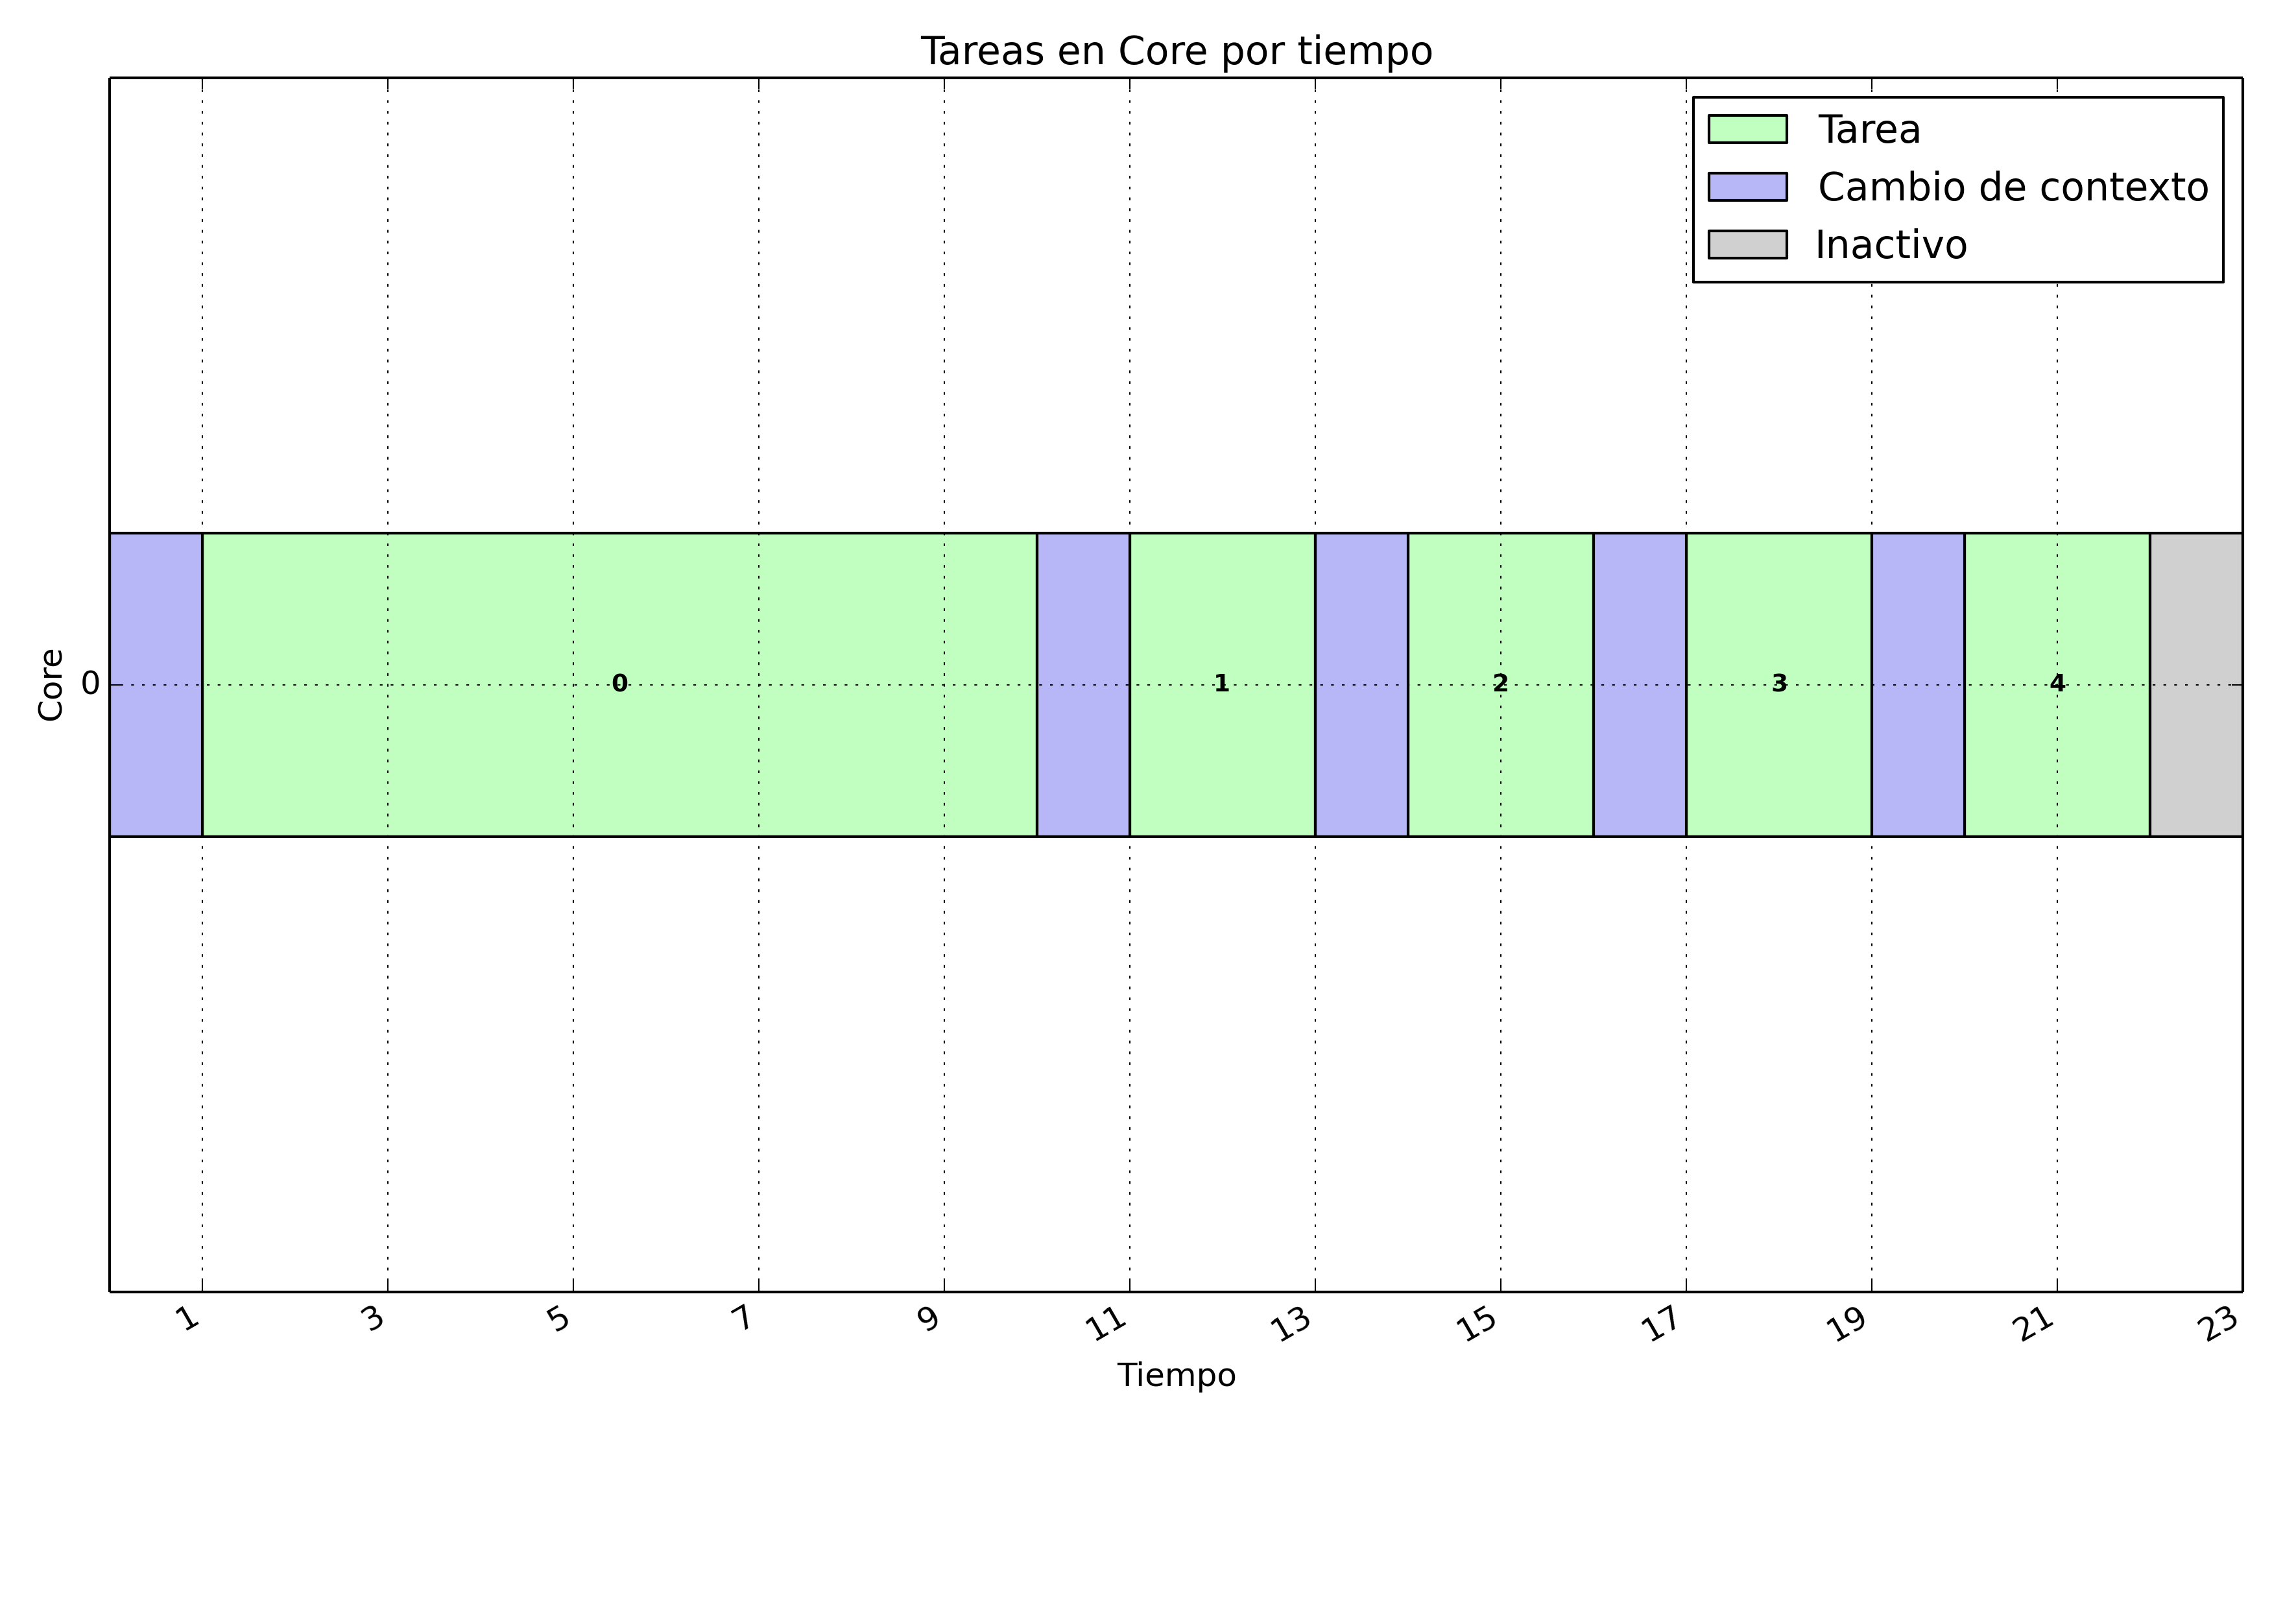
\includegraphics[width=\textwidth]{ejercicio_9_1}
\end{figure}

\begin{figure}[H]
\caption{Dynamic}
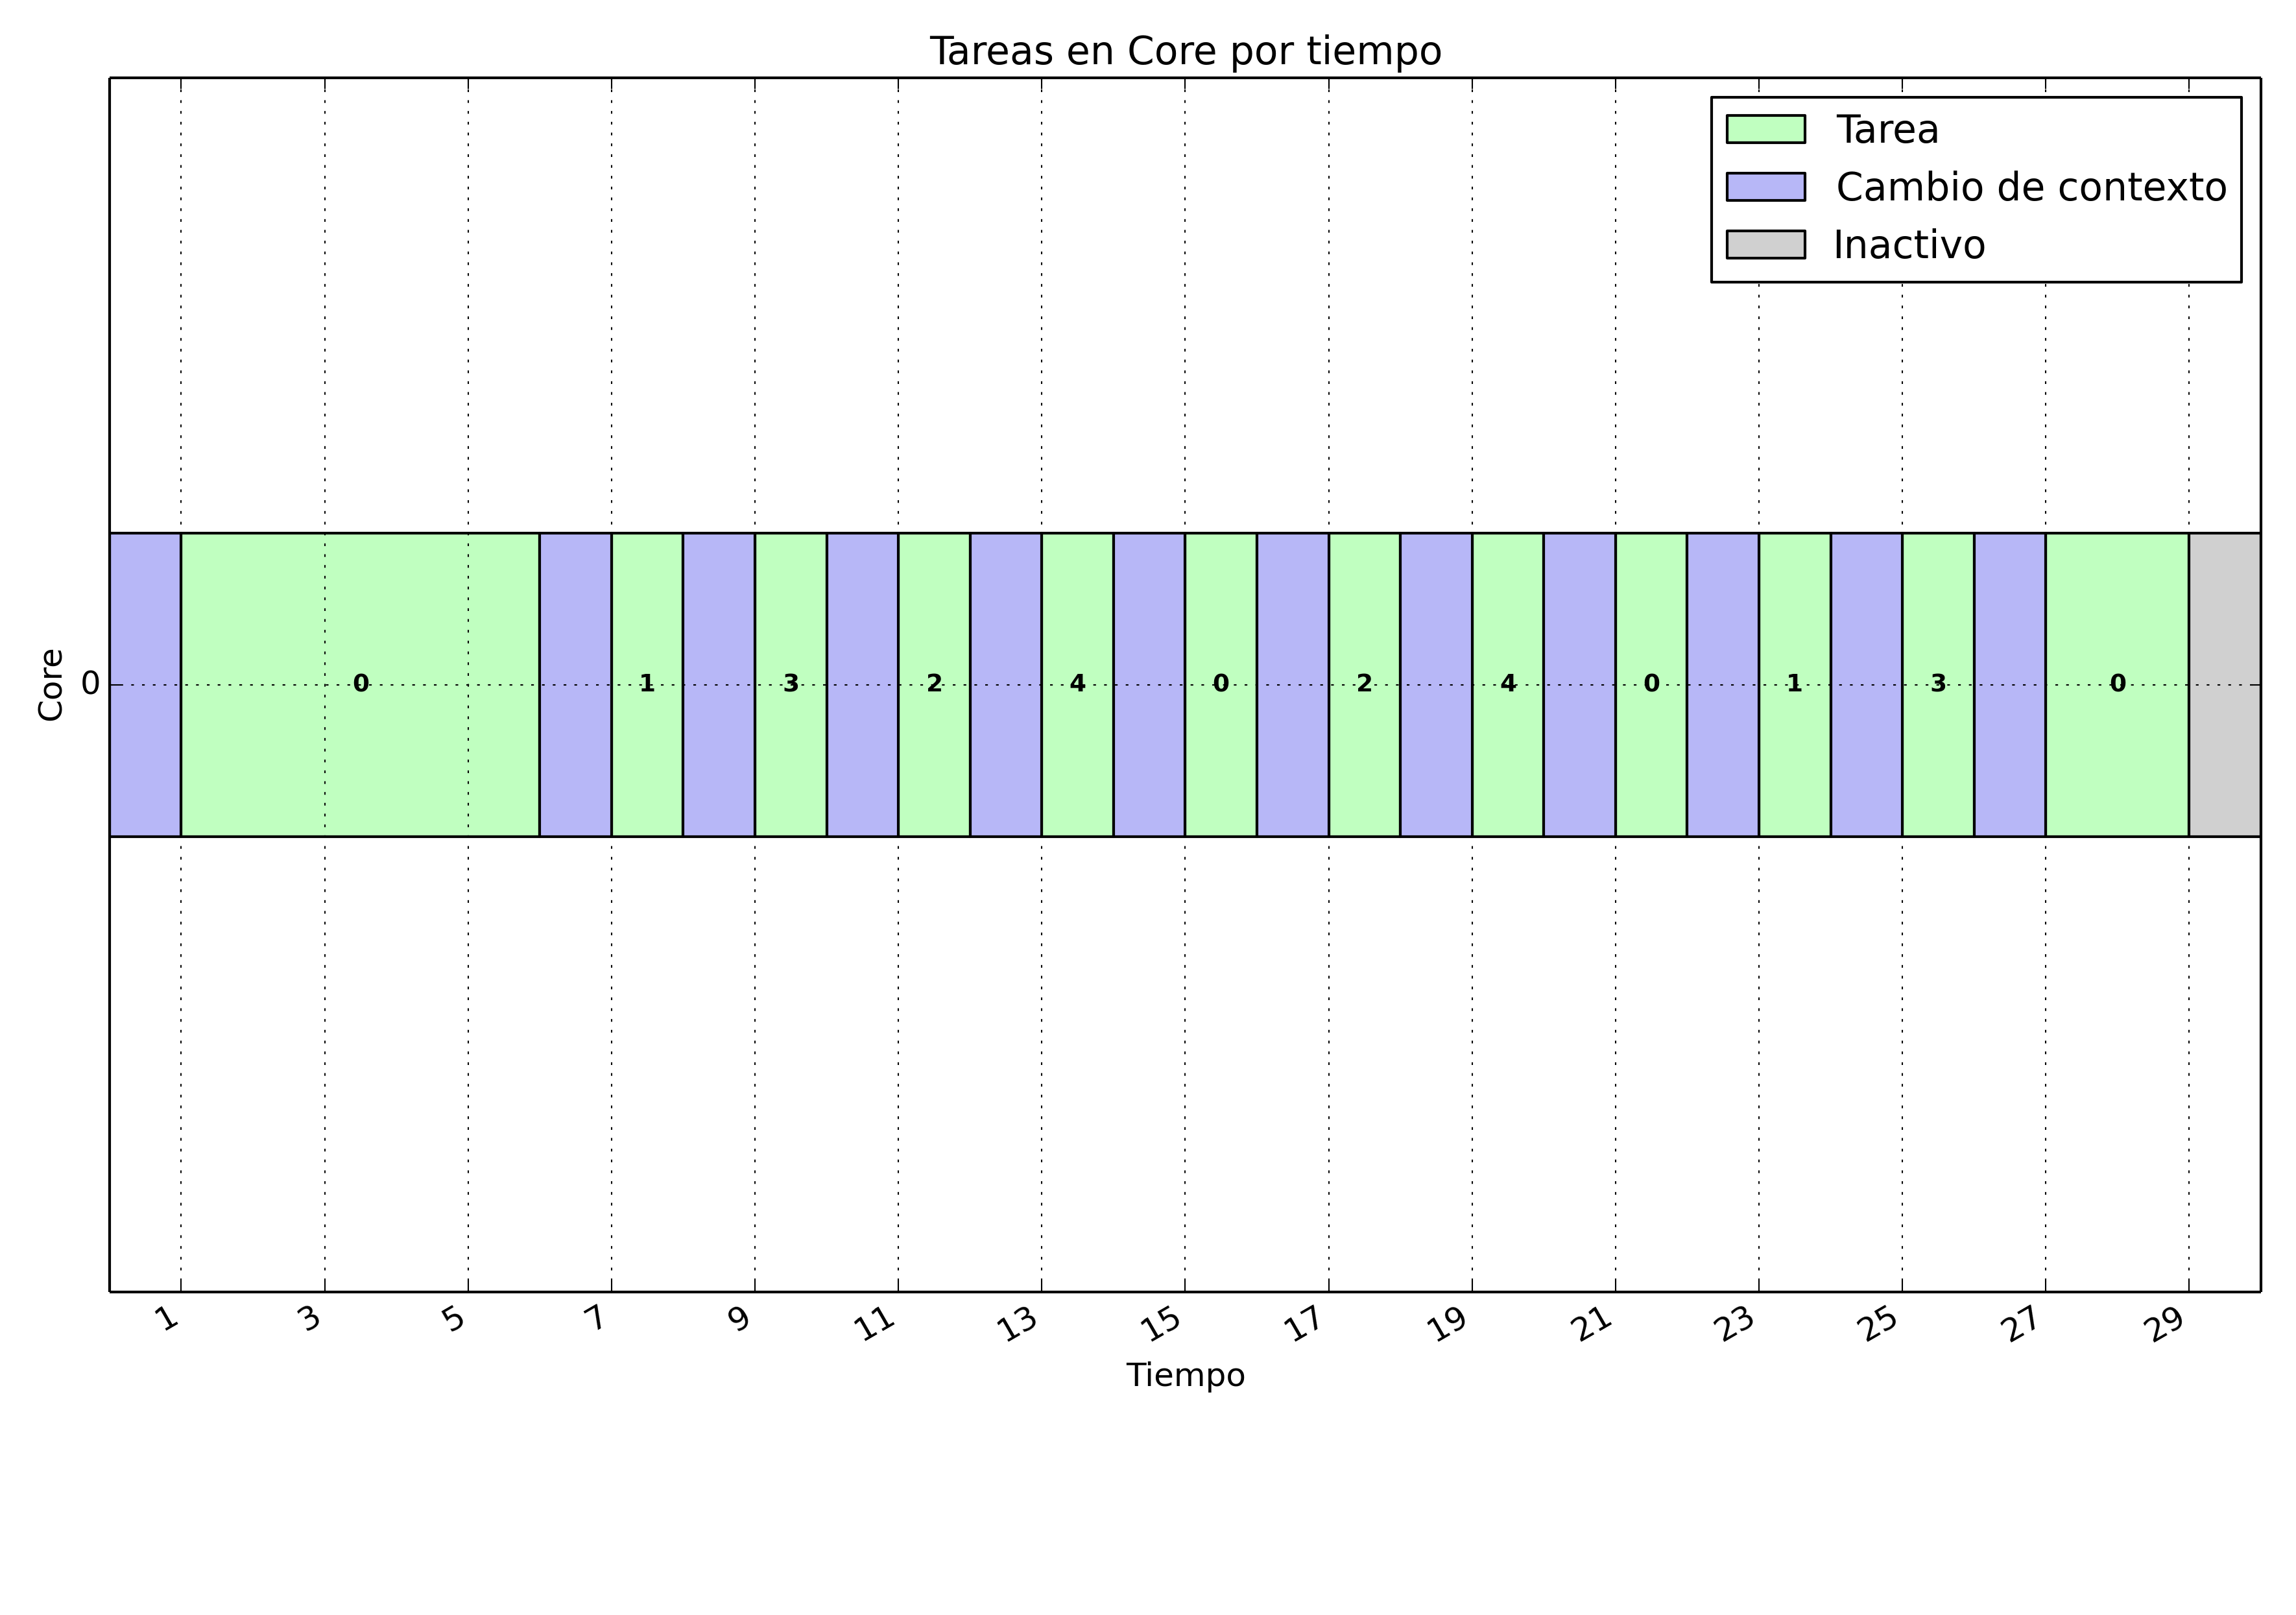
\includegraphics[width=\textwidth]{ejercicio_9_2}
\end{figure}

Se observa que en el caso del fixed se lleg\'o a un overflow para la tarea 0. Esto se produjo porque al ingresar las tareas de las familia B en el momento 6, fueron m\'as prioritarias en la medida en que ellas ten\'ian un request rate de $1/8$, mientras que el request rate de la tarea de la familia A era de $1/10$. 

Sin embargo, en el caso de la estrategia din\'amica no se produce el overflow porque al ingresar al sistema las tareas de la familia B, la tarea 0 sigue siendo m\'as prioritaria ya que su deadline se encuentra m\'as cercano.